\documentclass[12pt,a4paper,twoside,openright]{report}
\let\openright=\cleardoublepage



%%% Choose a language %%%

\newif\ifEN
% \ENtrue   % uncomment this for english
\ENfalse   % uncomment this for czech

%%% Configuration of the title page %%%

\def\ThesisTitleStyle{mff} % MFF style
%\def\ThesisTitleStyle{cuni} % uncomment for old-style with cuni.cz logo
%\def\ThesisTitleStyle{natur} % uncomment for nature faculty logo

\def\UKFaculty{Faculty of Mathematics and Physics}
%\def\UKFaculty{Faculty of Science}

\def\UKName{Charles University in Prague} % this is not used in the "mff" style

% Thesis type names, as used in several places in the title
\def\ThesisTypeTitle{\ifEN BACHELOR THESIS \else BAKALÁŘSKÁ PRÁCE \fi}
%\def\ThesisTypeTitle{\ifEN MASTER THESIS \else DIPLOMOVÁ PRÁCE \fi}
%\def\ThesisTypeTitle{\ifEN RIGOROUS THESIS \else RIGORÓZNÍ PRÁCE \fi}
%\def\ThesisTypeTitle{\ifEN DOCTORAL THESIS \else DISERTAČNÍ PRÁCE \fi}
\def\ThesisGenitive{\ifEN bachelor \else bakalářské \fi}
%\def\ThesisGenitive{\ifEN master \else diplomové \fi}
%\def\ThesisGenitive{\ifEN rigorous \else rigorózní \fi}
%\def\ThesisGenitive{\ifEN doctoral \else disertační \fi}
\def\ThesisAccusative{\ifEN bachelor \else bakalářskou \fi}
%\def\ThesisAccusative{\ifEN master \else diplomovou \fi}
%\def\ThesisAccusative{\ifEN rigorous \else rigorózní \fi}
%\def\ThesisAccusative{\ifEN doctoral \else disertační \fi}



%%% Fill in your details %%%

% (Note: \xxx is a "ToDo label" which makes the unfilled visible. Remove it.)
\def\ThesisTitle{Možnosti návrhového vzoru Entity-Component-System: případová studie}
\def\ThesisAuthor{Petr Kotáb}
\def\YearSubmitted{2024}

% department assigned to the thesis
\def\Department{Katedra softwaru a výuky informatiky}
% Is it a department (katedra), or an institute (ústav)?
\def\DeptType{Katedra}

\def\Supervisor{Mgr. Pavel Ježek, Ph.D.}
\def\SupervisorsDepartment{Katedra distribuovaných a spolehlivých systémů}

% Study programme and specialization
\def\StudyProgramme{Informatika }
\def\StudyBranch{Počítačová grafika, vidění a vývoj her}

\def\Dedication{%
Dedication. \xxx{It is nice to say thanks to supervisors, friends, family, book authors and food providers.}
}

\def\AbstractEN{%
\xxx{Abstracts are an abstract form of art. Use the most precise, shortest sentences that state what problem the thesis addresses, how it is approached, pinpoint the exact result achieved, and describe the applications and significance of the results. Highlight anything novel that was discovered or improved by the thesis. Maximum length is 200 words, but try to fit into 120. Abstracts are often used for deciding if a reviewer will be suitable for the thesis; a well-written abstract thus increases the probability of getting a reviewer who will like the thesis.}
% ABSTRACT IS NOT A COPY OF YOUR THESIS ASSIGNMENT!
}

\def\AbstractCS{%
\xxx{You will need to submit both Czech and English abstract to the SIS, no matter what language you use in the thesis. If writing in English, translate the contents of \texttt{\textbackslash{}AbstractEN} into this field. In case you do not speak czech, your supervisor should be able to help you with the translation.}
}

% 3 to 5 keywords (recommended), each enclosed in curly braces.
% Keywords are useful for indexing and searching for the theses by topic.
\def\Keywords{
    {návrhový vzor}
    {Entity-Component-System}
    {počítačové hry}
    {simulace}
    {případová studie}
}

% If your abstracts are long and do not fit in the infopage, you can make the
% fonts a bit smaller by this setting. (Also, you should try to compress your abstract more.)
% Alternatively, consider increasing the size of the page by uncommenting the
% geometry modification in thesis.tex.
\def\InfoPageFont{}
%\def\InfoPageFont{\small}  %uncomment to decrease font size

\ifEN\relax\else
% If you are writing a czech thesis, you additionally need to fill in the
% english translation of the metadata here!
\def\ThesisTitleEN{Exploring Options of Entity-Component-System Design Pattern: A Case Study}
\def\DepartmentEN{Department of software and computer science education}
\def\DeptTypeEN{Department}
\def\SupervisorsDepartmentEN{Department of Distributed and Dependable Systems}
\def\StudyProgrammeEN{Computer Science}
\def\StudyBranchEN{Computer Graphics, Vision and Game Development}
\def\KeywordsEN{
    {design pattern}
    {Entity-Component-System}
    {computer games}
    {simulation}
    {case study}
}
\fi


\usepackage[a-2u]{pdfx}

\ifEN\else\usepackage[czech,shorthands=off]{babel}\fi

% See https://en.wikipedia.org/wiki/Canons_of_page_construction before
% modifying the size of printable area. LaTeX defaults are great.
% If you feel it would help anything, you can enlarge the printable area a bit:
%\usepackage[textwidth=390pt,textheight=630pt]{geometry}
% The official recommendation expands the area quite a bit (looks pretty harsh):
%\usepackage[textwidth=145mm,textheight=247mm]{geometry}

%%% TYPICAL FONT CHOICES (uncomment what you like) %%%
% Recommended combo: Libertinus (autoselects Biolinum for sans) and everything
% else (math+tt) comes from Latin Modern)
\usepackage{lmodern}
\usepackage[mono=false]{libertinus}

% For the "classic" LaTeX fonts (very good for pure math theses), simply
% comment out the libertinus package above.

% IBM Plex font suite: nice, but requires us to fine-tune the sizes and does
% not directly support small caps (\textsc):
%\usepackage[usefilenames,RM={Scale=0.88},SS={Scale=0.88},SScon={Scale=0.88},TT={Scale=0.88},DefaultFeatures={Ligatures=Common}]{plex-otf}

% TeX Gyre combo (Pagella+Heros+Cursor)
%\usepackage{fontspec}
%\setmainfont{TeX Gyre Pagella}
%\setsansfont{TeX Gyre Heros}
%\setmonofont{TeX Gyre Cursor}

% some useful packages
\usepackage{microtype}
\usepackage{amsmath,amsfonts,amsthm,bm}
\usepackage{graphicx}
\usepackage{xcolor}
\usepackage{booktabs}
\usepackage{caption}
\usepackage{floatrow}

% Bibliography formatting.
% CHECK THE REQUIREMENTS OF YOUR DEPARTMENT AND FACULTY ON THE CITATION FORMAT!
%
% These are relatively "safe" default options that most people use:
\usepackage[natbib,style=numeric,sorting=none]{biblatex}
% alternative with alphanumeric citations (more informative than numbers, and
% more common in computer science journals):
%\usepackage[natbib,style=alphabetic]{biblatex}
%
% ALTERNATIVES THAT CONFORM TO ISO690
% ISO690 is not the greatest citation format ever, but may be formally
% required at Charles University, depending on your faculty and department.
%\usepackage[natbib,style=iso-numeric,sorting=none]{biblatex}
%\usepackage[natbib,style=iso-alphabetic]{biblatex}
% You might want to add extra options such as `maxbibnames=6,maxcitenames=2`
% here to further conform to some of the formatting requirements (see below for
% details). Again, consult your faculty rules.
%
% Additional option choices:
%  - add `giveninits=true` to typeset "E. A. Poe" instead of full Edgar Allan
%  - `terseinits=true` additionaly shortens it to nature-like "Poe EA"
%  - add `maxnames=10` to limit (or loosen) the maximum number of authors in
%    bibliography entry before shortening to `et al.` (useful when referring to
%    book collections that may have hundreds of authors)
%  - use `maxcitenames=2` to finetune the amount of authors listed in text-cite
%    commands (\citet). Corresponding option that only affects the bibliography
%    is `maxbibnames=10`.
%  - `sorting=none` causes the bibliography list to be ordered by the order of
%    citation as they appear in the text, which is usually the desired behavior
%    with numeric citations. Additionally you can use a style like
%    `numeric-comp` that compresses the long lists of citations such as
%    [1,2,3,4,5,6,7,8] to simpler [1--8]. This is especially useful if you plan
%    to add tremendous amounts of citations, as usual in life sciences and
%    bioinformatics.
%  - if you don't like the "In:" appearing in the bibliography, use the
%    extended style (`ext-numeric` or `ext-alphabetic`), and add option
%    `articlein=false`.
%
% possibly reverse the names of the authors with the default styles:
%\DeclareNameAlias{default}{family-given}

% load the file with bibliography entries
\addbibresource{refs.bib}

% remove this if you won't use fancy verbatim environments
\usepackage{fancyvrb}

% remove this if you won't typeset TikZ graphics
\usepackage{tikz}
\usetikzlibrary{positioning} %add libraries as needed (shapes, decorations, ...)

% remove this if you won't typeset any pseudocode
\usepackage{algpseudocode}
\usepackage{algorithm}

% remove this if you won't list any source code
\usepackage{listings}


\hypersetup{unicode}
\hypersetup{breaklinks=true}

\usepackage[noabbrev]{cleveref}


% various forms of TODOs (you should remove this before submitting)
\usepackage[textsize=tiny, backgroundcolor=yellow!25, linecolor=black!25]{todonotes}
\newcommand{\xxx}[1]{\textcolor{red!}{#1}}

 % remove this before compiling the final version


% use this for typesetting a chapter without a number, e.g. intro and outro
\def\chapwithtoc#1{\chapter*{#1}\addcontentsline{toc}{chapter}{#1}}

% If there is a line/figure overflowing into page margin, this will make the
% problem evident by drawing a thick black line at the overflowing spot. You
% should not disable this.
\overfullrule=3mm

% The maximum stretching of a space. Increasing this makes the text a bit more
% sloppy, but may prevent the overflows by moving words to next line.
\emergencystretch=1em

\ifEN
\theoremstyle{plain}
\newtheorem{thm}{Theorem}
\newtheorem{lemma}[thm]{Lemma}
\newtheorem{claim}[thm]{Claim}
\newtheorem{defn}{Definition}
\theoremstyle{remark}
\newtheorem*{cor}{Corollary}
\else
\theoremstyle{plain}
\newtheorem{thm}{Věta}
\newtheorem{lemma}{Lemma}
\newtheorem{claim}{Tvrzení}
\newtheorem{defn}{Definice}
\theoremstyle{remark}
\newtheorem*{cor}{Důsledek}
\fi

\newenvironment{myproof}{
  \par\medskip\noindent
  \textit{\ifEN Proof \else Důkaz \fi}.
}{
\newline
\rightline{$\qedsymbol$}
}

% real/natural numbers
\newcommand{\R}{\mathbb{R}}
\newcommand{\N}{\mathbb{N}}

% asymptotic complexity
\newcommand{\asy}[1]{\mathcal{O}(#1)}

% listings and default lstlisting config (remove if unused)
\DeclareNewFloatType{listing}{}
\floatsetup[listing]{style=ruled}

\DeclareCaptionStyle{thesis}{style=base,font={small,sf},labelfont=bf,labelsep=quad}
\captionsetup{style=thesis}
\captionsetup[algorithm]{style=thesis,singlelinecheck=off}
\captionsetup[listing]{style=thesis,singlelinecheck=off}

% Customization of algorithmic environment (comment style)
\renewcommand{\algorithmiccomment}[1]{\textcolor{black!25}{\dotfill\sffamily\itshape#1}}

% Uncomment for table captions on top. This is sometimes recommended by the
% style guide, and even required for some publication types.
%\floatsetup[table]{capposition=top}
%
% (Opinionated rant:) Captions on top are not "compatible" with the general
% guideline that the tables should be formatted to be quickly visually
% comprehensible and *beautiful* in general (like figures), and that the table
% "head" row (with column names) should alone communicate most of the content
% and interpretation of the table. If you just need to show a long boring list
% of numbers (because you have to), either put some effort into showing the
% data in an attractive figure-table, or move the data to an attachment and
% refer to it, so that the boredom does not impact the main text flow.
%
% You can make the top-captions look much less ugly by aligning the widths of
% the caption and the table, with setting `framefit=yes`, as shown below.  This
% additionally requires some extra markup in your {table} environments; see the
% comments in the example table in `ch2.tex` for details.
%\floatsetup[table]{capposition=top,framefit=yes}

\ifEN\floatname{listing}{Listing}
\else\floatname{listing}{Výpis kódu}\fi
\lstset{ % use this to define styling for any other language
  language=C++,
  tabsize=2,
  showstringspaces=false,
  basicstyle=\footnotesize\tt\color{black!75},
  identifierstyle=\bfseries\color{black},
  commentstyle=\color{green!50!black},
  stringstyle=\color{red!50!black},
  keywordstyle=\color{blue!75!black}}

% Czech versions of the used cleveref references (It's not as convenient as in
% English because of declension, cleveref is limited to sg/pl nominative. Use
% plain \ref to dodge that.)
\ifEN\relax\else
\crefname{chapter}{kapitola}{kapitoly}
\Crefname{chapter}{Kapitola}{Kapitoly}
\crefname{section}{sekce}{sekce}
\Crefname{section}{Sekce}{Sekce}
\crefname{subsection}{sekce}{sekce}
\Crefname{subsection}{Sekce}{Sekce}
\crefname{subsubsection}{sekce}{sekce}
\Crefname{subsubsection}{Sekce}{Sekce}
\crefname{figure}{obrázek}{obrázky}
\Crefname{figure}{Obrázek}{Obrázky}
\crefname{table}{tabulka}{tabulky}
\Crefname{table}{Tabulka}{Tabulky}
\crefname{listing}{výpis}{výpisy}
\Crefname{listing}{Výpis}{Výpisy}
\floatname{algorithm}{Algoritmus}
\crefname{algorithm}{algoritmus}{algoritmy}
\Crefname{algorithm}{Algoritmus}{Algoritmy}
\newcommand{\crefpairconjunction}{ a~}
\newcommand{\crefrangeconjunction}{ a~}
\fi
 % use this file for various custom definitions


\begin{document}

% the layout is mandatory, edit only in dire circumstances

\pagestyle{empty}
\hypersetup{pageanchor=false}
\begin{center}

% top part of the layout, this actually differs between faculties

\def\ThesisTitleXmff{%
  \ifEN
    \centerline{\mbox{
\includegraphics[width=166mm]{img/logo-en.pdf}}}
  \else
    \centerline{\mbox{
\includegraphics[width=166mm]{img/logo-cs.pdf}}}
  \fi
  \vspace{-8mm}\vfill%
  {\bf\Large\ThesisTypeTitle}
  \vfill%
  {\LARGE\ThesisAuthor}\par
  \vspace{15mm}%
  {\LARGE\bfseries\ThesisTitle}
  \vfill%
  \Department}
\def\ThesisTitleCuniLogo#1{%
  {\large\UKName\par\medskip\par\UKFaculty }
  \vfill%
  {\bf\Large\ThesisTypeTitle}
  \vfill%
  \includegraphics[width=70mm]{#1}
  \vfill%
  {\LARGE\ThesisAuthor}\par
  \vspace{15mm}%
  {\LARGE\bfseries\ThesisTitle}
  \vfill%
  \Department\par}
\def\ThesisTitleXcuni{\ThesisTitleCuniLogo{img/uklogo.pdf}}
\def\ThesisTitleXnatur{\ThesisTitleCuniLogo{img/naturlogo.pdf}}

% choose the correct page and print it
\csname ThesisTitleX\ThesisTitleStyle\endcsname
% latex corner: X is the new @

\vfill

{
\centerline{\vbox{\halign{\hbox to 0.45\hsize{\hfil #}&\hskip 0.5em\parbox[t]{0.45\hsize}{\raggedright #}\cr
\ifEN Supervisor of the \ThesisGenitive thesis:
\else Vedoucí \ThesisGenitive práce: \fi
& \Supervisor \cr
\noalign{\vspace{2mm}}
\ifEN Study programme: \else Studijní program: \fi
& \StudyProgramme \cr
\noalign{\vspace{2mm}}
\ifEN Study branch: \else Studijní obor: \fi
& \StudyBranch \cr
}}}}

\vfill

\ifEN Prague \else Praha \fi
\YearSubmitted

\end{center}

\newpage

% remember to sign this!
\openright
\hypersetup{pageanchor=true}
\pagestyle{plain}
\pagenumbering{roman}
\vglue 0pt plus 1fill

\ifEN
\noindent
I declare that I carried out this \ThesisAccusative thesis independently, and only with the cited
sources, literature and other professional sources. It has not been used to obtain another
or the same degree.
\else
\noindent
Prohlašuji, že jsem tuto \ThesisAccusative práci vypracoval(a) samostatně a výhradně
s~použitím citovaných pramenů, literatury a dalších odborných zdrojů.
Tato práce nebyla využita k získání jiného nebo stejného titulu.
\fi

\ifEN
\medskip\noindent
I understand that my work relates to the rights and obligations under the Act No.~121/2000 Sb.,
the Copyright Act, as amended, in particular the fact that the Charles
University has the right to conclude a license agreement on the use of this
work as a school work pursuant to Section 60 subsection 1 of the Copyright~Act.
\else
\medskip\noindent
Beru na~vědomí, že se na moji práci vztahují práva a povinnosti vyplývající
ze zákona č. 121/2000 Sb., autorského zákona v~platném znění, zejména skutečnost,
že Univerzita Karlova má právo na~uzavření licenční smlouvy o~užití této
práce jako školního díla podle §60 odst. 1 autorského zákona.
\fi

\vspace{10mm}


\ifEN
\hbox{\hbox to 0.5\hsize{%
In \hbox to 6em{\dotfill} date \hbox to 6em{\dotfill}
\hss}\hbox to 0.5\hsize{\dotfill\quad}}
\smallskip
\hbox{\hbox to 0.5\hsize{}\hbox to 0.5\hsize{\hfil Author's signature\hfil}}
\else
\hbox{\hbox to 0.5\hsize{%
V \hbox to 6em{\dotfill} dne \hbox to 6em{\dotfill}
\hss}\hbox to 0.5\hsize{\dotfill\quad}}
\smallskip
\hbox{\hbox to 0.5\hsize{}\hbox to 0.5\hsize{\hfil Podpis autora\hfil}}
\fi

\vspace{20mm}
\newpage

% dedication

\openright

\noindent
\Dedication

\newpage

% mandatory information page

\openright

\vbox to 0.49\vsize{\InfoPageFont
\setlength\parindent{0mm}
\setlength\parskip{5mm}

\ifEN Title: \else Název práce: \fi
\ThesisTitle

\ifEN Author: \else Autor: \fi
\ThesisAuthor

\DeptType:
\Department

\ifEN Supervisor: \else Vedoucí \ThesisGenitive práce: \fi
\Supervisor, \SupervisorsDepartment

\ifEN Abstract: \AbstractEN \else Abstrakt: \AbstractCS \fi

\ifEN Keywords: \else Klíčová slova: \fi
\Keywords

\vss}\ifEN\relax\else\nobreak\vbox to 0.49\vsize{\InfoPageFont
\setlength\parindent{0mm}
\setlength\parskip{5mm}

Title:
\ThesisTitleEN

Author:
\ThesisAuthor

\DeptTypeEN:
\DepartmentEN

Supervisor:
\Supervisor, \SupervisorsDepartmentEN

Abstract:
\AbstractEN

Keywords:
\KeywordsEN

\vss}
\fi

\newpage

\openright
\pagestyle{plain}
\pagenumbering{arabic}
\setcounter{page}{1}


\tableofcontents

\chapter{Úvod}
Vytváření her představuje komplexní proces, který zahrnuje mnoho fází prototypování a iterací. Často se dostáváme do situace, kdy je nezbytné výrazně upravit již existující kód. Z tohoto důvodu je klíčová vysoká flexibilita architektury kódu. Jeden z přístupů k řešení tohoto problému je využít návrhový vzor Component, který s sebou nese vysokou míru flexibility.

Nicméně v této práci se zaměříme na jiný přístup, konkrétně na návrhový vzor Entity-Component-System (ECS). Tento přístup nejenže poskytuje vysokou flexibilitu, ale také vyniká v oblasti výkonu. Mezi cíle této práce bude patřit prozkoumat možnosti, které tento návrhový vzor přináší, a ukázat výhody, které nám ECS může poskytnout v porovnání s návrhovým vzorem Component.

Abychom mohli efektivně využívat návrhový vzor ECS, je nezbytné implementovat odpovídající infrastrukturu. Samotná implementace této infrastruktury představuje obtížnou a časově náročnou úlohu, což vede mnoho vývojářů k volbě již existujících knihoven implementujících infrastrukturu pro tento návrhový vzor. Existuje však velké množství těchto knihoven, ale naštěstí existují měření, která nám mohou pomoci s výběrem takové knihovny.

Většina těchto měření provádí výkonnostní porovnání různých ECS knihoven prostřednictvím jednoduchých testů. Je třeba však zdůraznit, že v případě rozsáhlejšího projektu, jako je hra, se výsledky mohou lišit. Hlavním cílem této práce proto bude vytvoření rozsáhlejší hry, která nejenže napomůže plnit výše zmíněné cíle, ale také umožní srovnávat různé knihovny poskytující implementaci tohoto návrhového vzoru. Konkrétně budeme srovnávat knihovny pro programovací jazyk C\#, neboť se jedná o programovací jazyk běžně používaný pro hry a aplikace, a zajímá nás, jaká je situace těchto knihoven pro tento konkrétní programovací jazyk.

\section{Entity-Component-System}
Entity-Component-System (ECS) je návrhový vzor často používaný při vývoji her. Jeho základními stavebními kameny jsou entity, komponenty a systémy.
\begin{enumerate}
    \item \textbf{Entita (Entity):} Reprezentuje objekt v herní scéně. Může to být cokoliv, od hráče po strom nebo zvíře.
    \item \textbf{Komponenta (Component):} Entita je složena z komponent, které ji popisují. Komponenty obsahují pouze data a žádnou herní logiku. Například hráč může mít komponentu Control, která popisuje, jak se ovládá, strom může mít komponentu Resource, která popisuje, kolik dřeva hráč získá, pokud jej pokácí, a zvíře může mít komponentu PathFollow, která popisuje cestu, po které se pohybuje. Všechny tři entity mohou mít komponentu Appearance, která popisuje jak daný objekt vypadá.
    \item \textbf{Systém (System):} Obsahuje herní logiku. Systémy pracují nad určitou množinou komponent. V každé iteraci vezmou všechny entity obsahující tuto množinu komponent a provedou nad nimi určité operace. Například:
    \begin{itemize}
        \item \textbf{InputSystem:} Pracuje nad entitami s komponenty Control a Position, řídí logiku jejich ovládání.
        \item \textbf{PathMovementSystem:} Pracuje nad entitami s komponenty PathFollow a Movement, řídí logiku jejich pohybu po cestě.
        \item \textbf{RenderSystem:} Pracuje nad entitami s komponentou Appearance a řídí logiku jejich vykreslení.
    \end{itemize}
\end{enumerate}
Návrhový vzor ECS umožňuje oddělit data od logiky, což usnadňuje úpravy a rozšíření hry. Díky tomu je také efektivní z hlediska výkonu, což je klíčové pro hry, kde rychlost a flexibilita jsou nezbytné.

\section{Abstrakční vrstva}
Vzhledem k tomu, že plánujeme využít plánovanou hru k porovnávání různých ECS knihoven, je nezbytné navrhnout hru tak, aby fungovala nezávisle na konkrétní ECS knihovně. S ohledem na odlišné API jednotlivých ECS knihoven je nezbytné vytvořit abstrakční vrstvu pro ECS. Pro každou knihovnu, kterou budeme chtít porovnávat, poskytneme implementaci této vrstvy. Samotná hra poté pracuje s touto abstrakční vrstvou. Vytvoření takovéto vrstvy představuje náročný úkol, navzdory podobnosti rozhraní jednotlivých ECS knihoven. Významný rozdíl spočívá v rozhraní systémů, které se výrazně liší mezi jednotlivými knihovnami.

\section{Cíle práce}
Pro shrnutí, tato práce bude mít následující cíle:
\begin{enumerate}
    \item[h1)] Vytvořit hru pomocí ECS, která bude nezávislá na konkrétní ECS knihovně.
    \item[h2)] Pomocí vytvořené hry porovnat relativní výkon populárních ECS knihoven pro programovací jazyk C\#.
\end{enumerate}
S využitím této hry také budeme chtít:
\begin{enumerate}
    \item[v1)] Prozkoumat možnosti návrhového vzoru ECS.
    \item[v2)] Ukázat výhody, které nám ECS může nabídnout oproti návrhovému vzoru Component.
\end{enumerate}














\iffalse
\chapwithtoc{Introduction}

Introduction should answer the following questions, ideally in this order:
\begin{enumerate}
\item What is the nature of the problem the thesis is addressing?
\item What is the common approach for solving that problem now?
\item How this thesis approaches the problem?
\item What are the results? Did something improve?
\item What can the reader expect in the individual chapters of the thesis?
\end{enumerate}

Expected length of the introduction is between 1--4 pages. Longer introductions may require sub-sectioning with appropriate headings --- use \texttt{\textbackslash{}section*} to avoid numbering (with section names like `Motivation' and `Related work'), but try to avoid lengthy discussion of anything specific. Any ``real science'' (definitions, theorems, methods, data) should go into other chapters.
\todo{You may notice that this paragraph briefly shows different ``types'' of `quotes' in TeX, and the usage difference between a hyphen (-), en-dash (--) and em-dash (---).}

It is very advisable to skim through a book about scientific English writing before starting the thesis. I can recommend `\citetitle{glasman2010science}' by \citet{glasman2010science}.
\fi
\chapter{Important first chapter}
\label{chap:refs}

First chapter usually builds the theoretical background necessary for readers to understand the rest of the thesis. You should summarize and reference a lot of existing literature and research.

You should use the standard \emph{citations}\todo{Use \textbackslash{}emph command like this, to highlight the first occurrence of an important word or term. Reader will notice it, and hopefully remember the importance.}.

\begin{description}
\item[Obtaining bibTeX citation] Go to Google Scholar\footnote{\url{https://scholar.google.com}}\todo{This footnote is an acceptable way to `cite' webpages or URLs. Documents without proper titles, authors and publishers generally do not form citations. For this reason, avoid citations of wikipedia pages.}, find the relevant literature, click the tiny double-quote button below the link, and copy the bibTeX entry.
\item[Saving the citation] Insert the bibTeX entry to the file \texttt{refs.bib}. On the first line of the entry you should see the short reference name --- from Scholar, it usually looks like \texttt{author2015title} --- you will use that to refer to the citation.
\item[Using the citation] Use the \verb|\cite| command to typeset the citation number correctly in the text; a long citation description will be automatically added to the bibliography at the end of the thesis. Always use a non-breakable space before the citing parenthesis to avoid unacceptable line breaks:
\begin{Verbatim}
Trees utilize gravity to invade ye
noble sires~\cite{newton1666apple}.
\end{Verbatim}
\item[Why should I bother with citations at all?] For two main reasons:
\begin{itemize}
\item You do not have to explain everything in the thesis; instead you send the reader to refer to details in some other literature. Use citations to simplify the detailed explanations.
\item If you describe something that already exists without using a citation, the reviewer may think that you \emph{claim} to have invented it. Expectably, they will demand academic correctness, and, from your perspective, being accused of plagiarism is not a good starting point for a successful defense. Use citations to identify the people who invented the ideas that you build upon.
\end{itemize}
\item[How many citations should I use?]
Cite any non-trivial building block or assumption that you use, if it is published in the literature. You do not have to cite trivia, such as the basic definitions taught in the introductory courses.

The rule of thumb is that you should read, understand and briefly review at least around 4 scientific papers. A thesis that contains less than 3 sound citations will spark doubt in reviewers.
\end{description}

There are several main commands for inserting citations, used as follows:
\begin{itemize}
\item \citet{knuth1979tex} described a great system for typesetting theses.
\item We are typesetting this thesis with \LaTeX, which is based on \TeX{} and METAFONT~\cite{knuth1979tex}.
\item \TeX{} was expanded to \LaTeX{} by \citet{lamport1994latex}, hence the name.
\item Revered are the authors of these systems!~\cite{knuth1979tex,lamport1994latex}
\end{itemize}

\section{Some extra assorted hints before you start writing English}

\paragraph{Word order}
Strictly adhere to the English word order rules. The sentences follow a fixed structure with a subject followed by a verb and an object (in this order). Exceptions to this rule must be handled specially, and usually separated by commas.

\paragraph{Sentence structure}
Do not write long sentences. One sentence should contain exactly one fact. Multiple facts should be grouped in a paragraph to communicate one coherent idea. Both the sentences and paragraphs should include various hints about their relation to the other ideas and paragraps. These are typically materialized as adverbs or short sentence parts that clarify the cause--outcome and target--method--result relationship of the sentences in a paragraph. Such `word glue' helps the readers to correctly draw the lines that hold their mental images of your thesis together, and ideally see the big picture of what you were trying to convey right from the first read.

Paragraphs are grouped in labeled sections for a sole purpose of making the navigation in the thesis easier. Do not use the headings as `names for paragraphs' --- the text should make perfect sense even if all headings are removed. If a section of your text contains one paragraph per heading, you might have wanted to write an explicit list instead.

Mind the rules for placing commas:
\begin{itemize}
\item Do not use the comma before subordinate clauses that begin with `that' (like this one). English does not use subordinate clauses as often as Slavic languages because the lack of a suitable word inflection method makes them hard to understand. In scientific English, try to avoid them as much as possible. Ask doubtfully whether each `which' and `when' is necessary --- most of these helper conjunctions can be removed by converting the clause to non-subordinate.

As an usual example, \xxx{\textit{`The sentence, which I wrote, seemed ugly.'}} is perfectly bad; slightly improved by \xxx{\textit{`The sentence that I wrote seemed ugly.'}}, which can be easily reduced to \textit{`The sentence I wrote seemed ugly.'}. A final version with added storytelling value could say \textit{`I wrote a sentence but it seemed ugly.'}
\item Use the \emph{Oxford comma} before `and' and `or' at the end of a longer, comma-separated list of items. Certainly use it to disambiguate any possible mixtures of conjunctions: \textit{`The car is available in red, red and green, and green versions.'} Remember that English `or' is typically understood more like `either this or that, but not both,' and the use of `and` is much more appropriate in cases such as possibility overviews and example listings (like in this sentence).
\item Consider placing extra commas around any parts of the sentence that break the usual word order, especially if they are longer than a single word.
\end{itemize}

\paragraph{Nouns}
Every noun needs a determiner (`a', `the', `my', `some', \dots); the exceptions to this rule, such as non-adjectivized names and indeterminate plural, are relatively scarce. Without a determiner, a noun can be easily mistaken for something completely different, such as an adjective or a verb.

Name all things with appropriate nouns to help both the reader and yourself, and do not hesitate to invent good names and labels for anything that you will refer to more than once. Proper naming will save you a lot of writing effort because you will not have to repeat descriptions such as \xxx{\textit{`the third output of the second benchmarked method of the improved set,'}} instead you may introduce a labeling that will allow you to say just something like \textit{`output M2\textsuperscript{+}-3'}. At the same time, this will reduce the risk that the reader will confuse the object with another one --- for illustration, the long version of the previous example might very easily confuse with the second output of the third method. The same also applies to methods descriptions, algorithms, programs, testing datasets, theorems, use-cases, challenges and other things. As an example, \xxx{\textit{`the algorithm that organizes the potatoes into appropriate buckets'}} shortens nicely as \textit{`the potato bucketer'} and may be labeled as a procedure \textsc{BucketPotatoes()}, and \xxx{\textit{`the issue where the robot crashes into a wall and takes significant time to return to the previous task'}} may be called just \textit{`the crash--recovery lag'}.

\paragraph{Verbs}
Although English can express a whopping 65 base verb tenses and their variants, scientific literature often suppresses this complexity and uses only several basic tenses where the meaning is clearly defined. Typically, you state facts in present simple (\textit{`Theorem 1 proves that Gadget B works as intended.'}), talk about previous work and experiments done in past simple (\textit{`We constructed Gadget B from Gizmo C, which was previously prepared by Tinkerer et al.'}), and identify achieved results in present perfect (\textit{`We have constructed Technology T.'}). Avoid using future tense, except for sections that explicitly describe future work --- as a typical mistake, if you state that the thesis \emph{will} describe something in later chapters, you imply that the description is not present there yet.

Do not write sentences in passive voice, unless you explicitly need to highlight that something has passively subjected itself to an action. Active voice is more preferable in the theses because it clearly highlights the actors and their contributions --- typically, \textit{`you did it'} instead of \textit{`it was done'} by a mysterious entity, which the reviewers rarely envision as yourself. Writing in active voice additionally benefits the explanation of complex processes: There, the word order forces you to identify the acting subject as the first word in the sentence, which further disambiguates how the individual process parts are triggered and ordered.

Try to avoid overusing gerunds (verbs that end with `-ing'). It is convenient to write shorter sentences by using gerunds as adjectives, but these are typically quite hard to understand because the readers may easily confuse the intended adjectives with verbs. If your sentence contains two gerunds close to each other, it may need a rewrite.

\paragraph{Scientific writing resources}
Consult the book by \citet{glasman2010science} for more useful details and recommended terminology for writing about the scientific research. Very pragmatically, the book by \citet{sparling1989english} describes many common mistakes that Czech and Slovak (and generally Slavic) writers make when writing English.

\chapter{More complicated chapter}
\label{chap:math}

After the reader gained sufficient knowledge to understand your problem in \cref{chap:refs}, you can jump to your own advanced material and conclusions.

You will need definitions (see \cref{defn:x} below in \cref{sec:demo}), theorems (\cref{thm:y}), general mathematics, algorithms (\cref{alg:w}), and tables (\cref{tab:z})\todo{See documentation of package \texttt{booktabs} for hints on typesetting tables. As a main rule, \emph{never} draw a vertical line.}. \Cref{fig:f,fig:g} show how to make a nice figure. See \cref{fig:schema} for an example of TikZ-based diagram. Cross-referencing helps to keep the necessary parts of the narrative close --- use references to the previous chapter with theory wherever it seems that the reader could have forgotten the required context. Conversely, it is useful to add a few references to theoretical chapters that point to the sections which use the developed theory, giving the reader easy access to motivating application examples.

\section{Example with some mathematics}
\label{sec:demo}

\begin{defn}[Triplet]\label{defn:x}
Given stuff $X$, $Y$ and $Z$, we will write a \emph{triplet} of the stuff as $(X,Y,Z)$.
\end{defn}

\newcommand{\Col}{\textsc{Colour}}

\begin{thm}[Car coloring]\label{thm:y}
All cars have the same color. More specifically, for any set of cars $C$, we have
$$(\forall c_1, c_2 \in C)\:\Col(c_1) = \Col(c_2).$$
\end{thm}

\begin{proof}
Use induction on sets of cars $C$. The statement holds trivially for $|C|\leq1$. For larger $C$, select 2 overlapping subsets of $C$ smaller than $|C|$ (thus same-colored). Overlapping cars need to have the same color as the cars outside the overlap, thus also the whole $C$ is same-colored.\todo{This is plain wrong though.}
\end{proof}

\begin{table}
% uncomment the following line if you use the fitted top captions for tables
% (see the \floatsetup[table] comments in `macros.tex`.
%\floatbox{table}[\FBwidth]{
\centering\footnotesize\sf
\begin{tabular}{llrl}
\toprule
Column A & Column 2 & Numbers & More \\
\midrule
Asd & QWERTY & 123123 & -- \\
Asd qsd 1sd & \textcolor{red}{BAD} & 234234234 & This line should be helpful. \\
Asd & \textcolor{blue}{INTERESTING} & 123123123 & -- \\
Asd qsd 1sd & \textcolor{violet!50}{PLAIN WEIRD} & 234234234 & -- \\
Asd & QWERTY & 123123 & -- \\
\addlinespace % a nice non-intrusive separator of data groups (or final table sums)
Asd qsd 1sd & \textcolor{green!80!black}{GOOD} & 234234299 & -- \\
Asd & NUMBER & \textbf{123123} & -- \\
Asd qsd 1sd & \textcolor{orange}{DANGEROUS} & 234234234 & (no data) \\
\bottomrule
\end{tabular}
%}{  % uncomment if you use the \floatbox (as above), erase otherwise
\caption{An example table.  Table caption should clearly explain how to interpret the data in the table. Use some visual guide, such as boldface or color coding, to highlight the most important results (e.g., comparison winners).}
%}  % uncomment if you use the \floatbox
\label{tab:z}
\end{table}

\begin{figure}
\centering
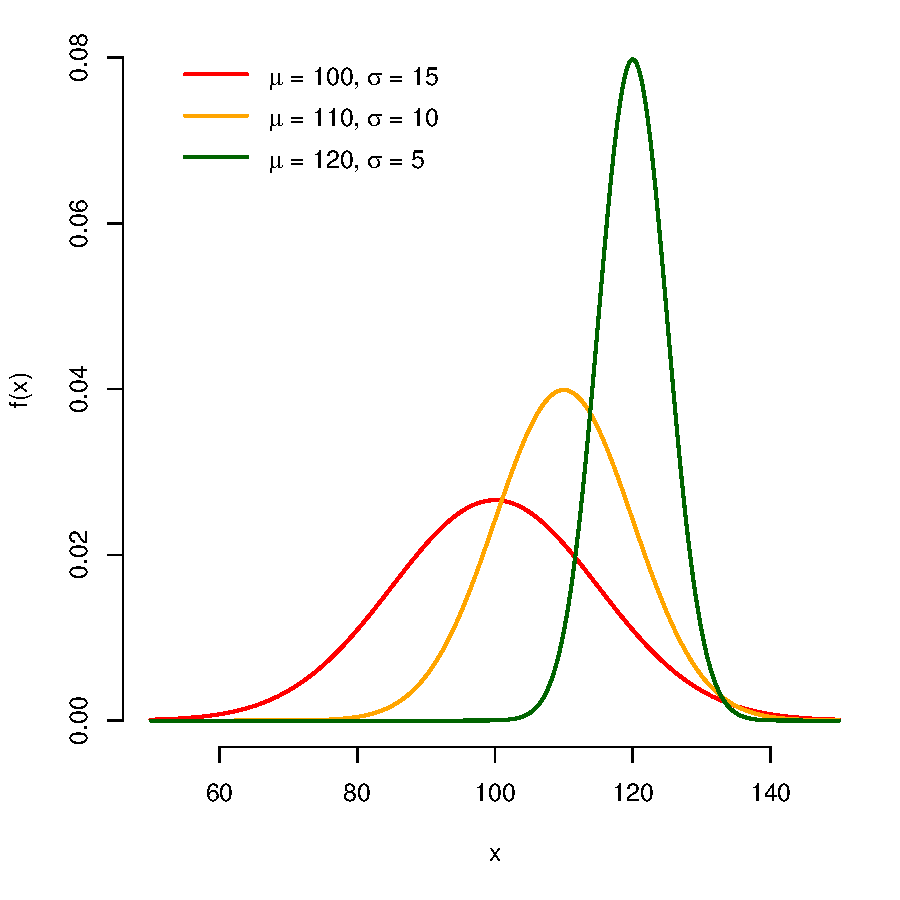
\includegraphics[width=.6\linewidth]{img/ukazka-obr02.pdf}
\caption{A figure with a plot, not entirely related to anything. If you copy the figures from anywhere, always refer to the original author, ideally by citation (if possible). In particular, this picture --- and many others, also a lot of surrounding code --- was taken from the example bachelor thesis of MFF, originally created by Martin Mareš and others.}
\label{fig:g}
\end{figure}

\begin{figure}
\centering
\tikzstyle{box}=[rectangle,draw,rounded corners=0.5ex,fill=green!10]
\begin{tikzpicture}[thick,font=\sf\scriptsize]
\node[box,rotate=45] (a) {A test.};
\node[] (b) at (4,0) {Node with no border!};
\node[circle,draw,dashed,fill=yellow!20, text width=6em, align=center] (c) at (0,4) {Ugly yellow node.\\Is this the Sun?};
\node[box, right=1cm of c] (d) {Math: $X=\sqrt{\frac{y}{z}}$};
\draw[->](a) to (b);
\draw[->](a) to[bend left=30] node[midway,sloped,anchor=north] {flow flows} (c);
\draw[->>>,dotted](b) to[bend right=30] (d);
\draw[ultra thick](c) to (d);

\end{tikzpicture}
\caption{An example diagram typeset with TikZ. It is a good idea to write diagram captions in a way that guides the reader through the diagram. Explicitly name the object where the diagram viewing should ``start''. Preferably, briefly summarize the connection to the parts of the text and other diagrams or figures. (In this case, would the tenative yellow Sun be described closer in some section of the thesis? Or, would there be a figure to detail the dotted pattern of the line?)}
\label{fig:schema}
\end{figure}

\begin{algorithm}
\begin{algorithmic}
\Function{ExecuteWithHighProbability}{$A$}
	\State $r \gets$ a random number between $0$ and $1$
	\State $\varepsilon \gets 0.0000000000000000000000000000000000000042$
	\If{$r\geq\varepsilon$}
		\State execute $A$ \Comment{We discard the return value}
	\Else
		\State print: \texttt{Not today, sorry.}
	\EndIf
\EndFunction
\end{algorithmic}
\caption{Algorithm that executes an action with high probability. Do not care about formal semantics in the pseudocode --- semicolons, types, correct function call parameters and similar nonsense from `realistic' languages can be safely omitted. Instead make sure that the intuition behind (and perhaps some hints about its correctness or various corner cases) can be seen as easily as possible.}
\label{alg:w}
\end{algorithm}

\section{Extra typesetting hints}

Do not overuse text formatting for highlighting various important parts of your sentences. If an idea cannot be communicated without formatting, the sentence probably needs rewriting anyway. Imagine the thesis being read aloud as a podcast --- the storytellers are generally unable to speak in boldface font.

Most importantly, do \underline{not} overuse bold text, which is designed to literally \textbf{shine from the page} to be the first thing that catches the eye of the reader. More precisely, use bold text only for `navigation' elements that need to be seen and located first, such as headings, list item leads, and figure numbers.

Use underline only in dire necessity, such as in the previous paragraph where it was inevitable to ensure that the reader remembers to never typeset boldface text manually again.

Use \emph{emphasis} to highlight the first occurrences of important terms that the reader should notice. The feeling the emphasis produces is, roughly, ``Oh my --- what a nicely slanted word! Surely i~expect it be important for the rest of the thesis!''

Finally, never draw a vertical line, not even in a table or around figures, ever. Vertical lines outside of the figures are ugly.

\chapter{Results and discussion}

You should have a separate chapter for presenting your results (generated by the stuff described previously, in our case in \cref{chap:math}). Remember that your work needs to be validated rigorously, and no one will believe you if you just say that `it worked well for you'.

Instead, try some of the following:
\begin{itemize}
\item State a hypothesis and prove it statistically
\item Show plots with measurements that you did to prove your results (e.g. speedup). Use either \texttt{R} and \texttt{ggplot}, or Python with \texttt{matplotlib} to generate the plots.\footnote{Honestly, the plots from \texttt{ggplot} look \underline{much} better.} Save them as PDF to avoid printing pixels (as in \cref{fig:f}).
\item Compare with other similar software/theses/authors/results, if possible
\item Show example source code (e.g. for demonstrating how easily your results can be used)
\item Include a `toy problem' for demonstrating the basic functionality of your approach and detail all important properties and results on that
\item Include clear pictures of `inputs' and `outputs' of all your algorithms, if applicable
\end{itemize}

\begin{figure}
\centering
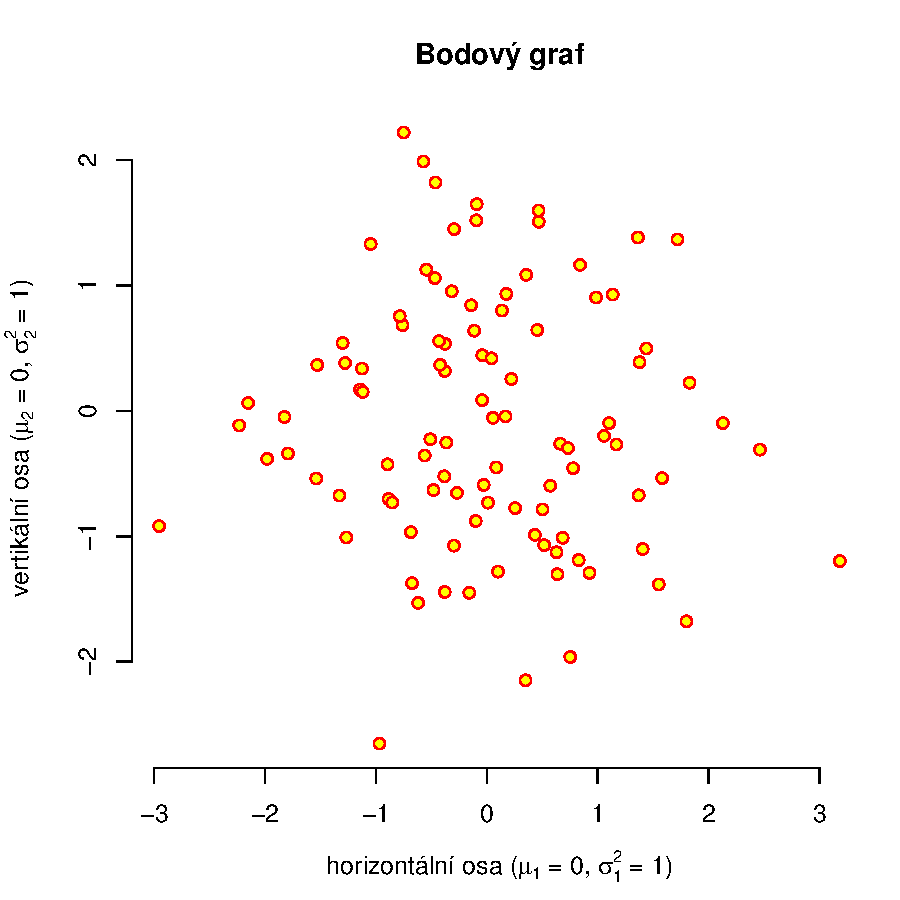
\includegraphics[width=.6\linewidth]{img/ukazka-obr01.pdf}
\caption{This caption is a friendly reminder to never insert figures ``in text,'' without a floating environment, unless explicitly needed for maintaining the text flow (e.g., the figure is small and developing with the text, like some of the centered equations, as in \cref{thm:y}). All figures \emph{must} be referenced by number from the text (so that the readers can find them when they read the text) and properly captioned (so that the readers can interpret the figure even if they look at it before reading the text --- reviewers love to do that).}
\label{fig:f}
\end{figure}

It is sometimes convenient (even recommended by some journals, including Cell) to name the results sub-sections so that they state what exactly has been achieved. Examples follow.

\section{SuperProgram is faster than OldAlgorithm}
\subsection{Scalability estimation}
\subsection{Precision of the results}
\section{Weird theorem is proven by induction}
\section{Amount of code reduced by CodeRedTool}
\subsection{Example}
\subsection{Performance on real codebases}
\section{\sloppy NeuroticHelper improves neural network learning}

\section{Graphics and figure quality}

No matter how great the text content of your thesis is, the pictures will always catch the attention first. This creates the very important first impression of the thesis contents and general quality. Crucially, that also decides whether the thesis is later read with joy, or carefully examined with suspicion.

Preparing your thesis in a way such that this first impression gets communicated smoothly and precisely helps both the reviewer and you: the reviewer will not have a hard time understanding what exactly you wanted to convey, and you will get a better grade.

Making the graphics `work for you' involves doing some extra work that is often unexpected. At the same time, you will need to fit into graphics quality constraints and guidelines that are rarely understood before you actually see a bad example. As a rule of thumb, you should allocate at least the same amount of time and effort for making the figures look good as you would for writing, editing and correcting the same page area of paragraph text.

\subsection{Visualize all important ideas}
The set of figures in your thesis should be comprehensive and complete. For all important ideas, constructions, complicated setups and results there should be a visualization that the reader can refer to in case the text does not paint the `mental image' sufficiently well. At the bare minimum, you should have at least 3 figures (roughly corresponding to the 3 chapters) that clearly and unambiguously show:
\begin{enumerate}
\item the context of the problem you are solving, optionally with e.g.~question marks and exclamation marks placed to highlight the problems and research questions
\item the overall architecture of your solution (usually as a diagram with arrows, such as in \cref{fig:schema}, ideally with tiny toy examples of the inputs and outputs of each box),
\item the advancement or the distinctive property of your solution, usually in a benchmark plot, or as a clear demonstration and comparison of your results.
\end{enumerate}

\subsection{Make the figures comprehensible}
The figures should be easily comprehensible. Surprisingly, that requires you to follow some common ``standards'' in figure design and processing. People are often used to a certain form of the visualizations, and (unless you have a very good reason) deviating from the standard is going to make the comprehension much more complicated. The common standards include the following:
\begin{itemize}
  \item caption everything correctly, place the caption at an expectable position
  \item systematically label the plots with `main' titles (usually in boldface, above the plot), plot axes, axis units and ticks, and legends
  \item lay out the diagrams systematically, ideally follow a structure of a bottom-up tree, a left-to-right pipeline, a top-down layered architecture, or a center-to-borders mindmap
  \item {use colors that convey the required information correctly \par\footnotesize Although many people carry some intuition for color use, achieving a really correct utilization of colors is often very hard without previous experience in color science and typesetting. Always remember that everyone perceives color hues differently, therefore the best distinction between the colors is done by varying lightness of the graphics elements (i.e., separating the data by dark vs.~light) rather than by using hues (i.e., forcing people to guess which one of salmon and olive colors means ``better''). Almost 10\% of the population have their vision impaired by some form of color vision deficiency, most frequently by deuteranomaly that prevents interpretation of even the most `obvious' hue differences, such as green vs.~red. Finally, printed colors look surprisingly different from the on-screen colors. You can prevent much of these problems by using standardized palettes and well-tested color gradients, such as the ones from ColorBrewer\footnote{\url{https://colorbrewer2.org}} and ViridisLite\footnote{\url{https://sjmgarnier.github.io/viridisLite/}}. Check if your pictures still look good if converted to greyscale, and use a color deficiency simulator to check how the colors are perceived with deuteranomaly.}
\end{itemize}

Avoid large areas of over-saturated and dark colors:
\begin{itemize}
  \item under no circumstances use dark backgrounds for any graphical elements, such as diagram boxes and tables --- use very light, slightly desaturated colors instead
  \item avoid using figures that contain lots of dark color (as a common example, heatmaps rendered with the `magma' color palette often look like huge black slabs that are visible even through the paper sheet, thus making a dark smudge on the neighboring page)
  \item increase the brightness of any photos to match the average brightness of the text around the figure
\end{itemize}

Remember to test your figures on other people --- usually, just asking `What do you think the figure should show?' can help you debug many mistakes in your graphics. If they think that the figure says something different than what you planned, then most likely it is your figure what is wrong, not the understanding of others.

Finally, there are many magnificent resources that help you arrange your graphics correctly. The two books by Tufte~\cite{tufte1990envisioning,tufte1983visual} are arguably classics in the area. Additionally, you may find many interesting resources to help you with technical aspects of plotting, such as the \texttt{ggplot}-style `Fundamentals' book by~\citet{wilke2019fundamentals}, and a wonderful manual for the TikZ/PGF graphics system by~\citet{tantau2015tikz} that will help you draw high-quality diagrams (like the one in~\cref{fig:schema}).

\section{What is a discussion?}
After you present the results and show that your contributions work, it is important to \emph{interpret} them, showing what they mean in the wider context of the thesis topic, for the researchers who work in the area, and for the more general public, such as for the users.

Separate discussion sections are therefore common in life sciences where some ambiguity in result interpretation is common, and the carefully developed intuition about the wider context is sometimes the only thing that the authors have. Exact sciences and mathematicians do not need to use the discussion sections as often. Despite of that, it is nice to position your output into the previously existing environment, answering:
\begin{itemize}
\item What is the potential application of the result?
\item Does the result solve a problem that other people encountered?
\item Did the results point to any new (surprising) facts?
\item How (and why) is the approach you chose different from what the others have done previously?
\item Why is the result important for your future work (or work of anyone other)?
\item Can the results be used to replace (and improve) anything that is used currently?
\end{itemize}

If you do not know the answers, you may want to ask the supervisor. Also, do not worry if the discussion section is half-empty or thoroughly pointless; you may remove it completely without much consequence. It is just a bachelor thesis, not a world-saving avenger thesis.


\chapwithtoc{Conclusion}

In the conclusion, you should summarize what was achieved by the thesis. In a few paragraphs, try to answer the following:
\begin{itemize}
\item Was the problem stated in the introduction solved? (Ideally include a list of successfully achieved goals.)
\item What is the quality of the result? Is the problem solved for good and the mankind does not need to ever think about it again, or just partially improved upon? (Is the incompleteness caused by overwhelming problem complexity that would be out of thesis scope\todo{This is quite common.}, or any theoretical reasons, such as computational hardness?)
\item Does the result have any practical applications that improve upon something realistic?
\item Is there any good future development or research direction that could further improve the results of this thesis? (This is often summarized in a separate subsection called `Future work'.)
\end{itemize}


\ifEN
\chapwithtoc{Bibliography}
\else
\chapwithtoc{Seznam použité literatury}
\fi

\printbibliography[heading=none]


\appendix
\chapter{Using CoolThesisSoftware}

Use this appendix to tell the readers (specifically the reviewer) how to use your software. A very reduced example follows; expand as necessary. Description of the program usage (e.g., how to process some example data) should be included as well.

To compile and run the software, you need dependencies XXX and YYY and a C compiler. On Debian-based Linux systems (such as Ubuntu), you may install these dependencies with APT:
\begin{Verbatim}
apt-get install \
  libsuperdependency-dev \
  libanotherdependency-dev \
  build-essential
\end{Verbatim}

To unpack and compile the software, proceed as follows:
\begin{Verbatim}
unzip coolsoft.zip
cd coolsoft
./configure
make
\end{Verbatim}

The program can be used as a C++ library, the simplest use is demonstrated in \cref{lst:ex}. A demonstration program that processes demonstration data is available in directory \verb|demo/|, you can run the program on a demonstration dataset as follows:
\begin{Verbatim}
cd demo/
./bin/cool_process_data data/demo1
\end{Verbatim}

After the program starts, control the data avenger with standard \verb-WSAD- controls.

\begin{listing}
\begin{lstlisting}
#include <CoolSoft.h>
#include <iostream>

int main() {
	int i;
	if(i = cool::ProcessAllData()) // returns 0 on error
		std::cout << i~<< std::endl;
	else
		std::cerr << "error!" << std::endl;
	return 0;
}
\end{lstlisting}
\caption{Example program.}
\label{lst:ex}
\end{listing}


% if your attachments are complicated, describe them in a separate appendix
%\chapwithtoc{Přílohy}
\label{chap:attachments}

\subsubsection{Přehled elektronických příloh}

\begin{enumerate}
    \item \texttt{src} -- Adresář obsahující zdrojové soubory a sestavený projekt měření. Součástí zdrojových souborů jsou dva projekty (WorldSimulator.csproj a WorldSimulator.Benchmarks.csproj).

    \item \texttt{build} -- Adresář obsahující sestavený projekt hry World Simulator.

    \item \texttt{README.md} -- Textový soubor obsahující opis seznamu příloh, dodatečné informace k seznamu příloh a kontakt na autora práce.
\end{enumerate}

\openright
\end{document}
